% Copyright (c) 2022 Tobias Briones. All rights reserved.
% SPDX-License-Identifier: CC-BY-SA-4.0
%
% This source code is part of
% https://github.com/tobiasbriones/cp-unah-is911-microprocessors and is
% licensed under the Creative Commons Attribution Share Alike 4.0
% International License found in the LICENSE file in the root
% directory of this source tree or at https://spdx.org/licenses/CC-BY-SA-4.0

\documentclass[conference]{IEEEtran}
\usepackage{preamble}

\title{ESP32 CON C++ Y MICOPHYTHON}
\author{
    
\includegraphics[width = 40mm]{images/logo-unah}\\[8ex]
    \IEEEauthorblockN{Tobias Briones}
    \IEEEauthorblockN{tobias.briones@unah.hn}
    \IEEEauthorblockA{\textit{Universidad Nacional Autónoma de Honduras} \\
    \textit{Ingeniería de Sistemas} \\
    \textit{I PAC 2022} \\
    \textit{IS911-MICROPROCESADORES}} \\\vspace*{20pt} \normalsize  \\
    \today
}

\begin{document}

    \maketitle

    \begin{abstract}

    \end{abstract}

    \tableofcontents

    \import{}{footer}

    \section{Introducción}\label{sec:introduction}

    ESP32 es una tarjeta microcontrolador de bajo costo \cite{wikipedia-esp32-2022} similar a las demás tarjetas conocidas como Arduino y Raspberry Pi Pico. Esta puede ser programada mediante Arduino IDE al hacer la configuración correspondiente y además mediante MicroPython también. Cuenta con una gran cantidad de características similares a las de este tipo de tarjetas microcontrolador de entrada.

    \bigbreak

    La tarjeta ESP32 tiene una gran capacidad de conexión inalámbrica tanto WiFi como Bluetooth, posee grandes integraciones en su diseño, bajo consumo de potencia y un diseño robusto \cite{espressif-systems-shanghai-co-ltd-2022A}. Por lo tanto, tenemos la siguiente denominación del producto:

    \bigbreak

    \begin{quote}
        Un MCU rico en funciones con Wi-Fi integrado y Conectividad Bluetooth para una amplia gama de aplicaciones.\\ \footnotesize
        Fuente: \textit{ESP32 Wi-Fi \& Bluetooth MCU} $\mid$ Espressif Systems \cite{espressif-systems-shanghai-co-ltd-2022A} (traducido de inglés a español, bajo uso justo)
    \end{quote}

    \bigbreak

    ESP32 es chip integrado con Wi-Fi y Bluetooth de $2.4GHz$ con la tecnología TSMC de ultra bajo poder de $40nm$, consiguiendo la mejor potencia y rendimiento de conectividad o de radiofrecuencia, así mismo como otros atributos tales como: robustez, versatilidad, y fiabilidad. Diseñado para ser un dispositivo móvil IoT con características específicas con estado del arte en este aspecto. \cite{espressif-systems-shanghai-co-ltd-2022B}.

    \bigbreak

    En la siguiente imágen se ve una tarjeta ESP32 montada en la tarjeta NodeMCU \footnote{Una tarjeta NodeMCU es una plataforma IoT de bajo costo y de código abierto que corre tarjetas ESP como la ESP32 \cite{wikipedia-mcu-2022B}}.

    \begin{figure}[H]
        \centering
        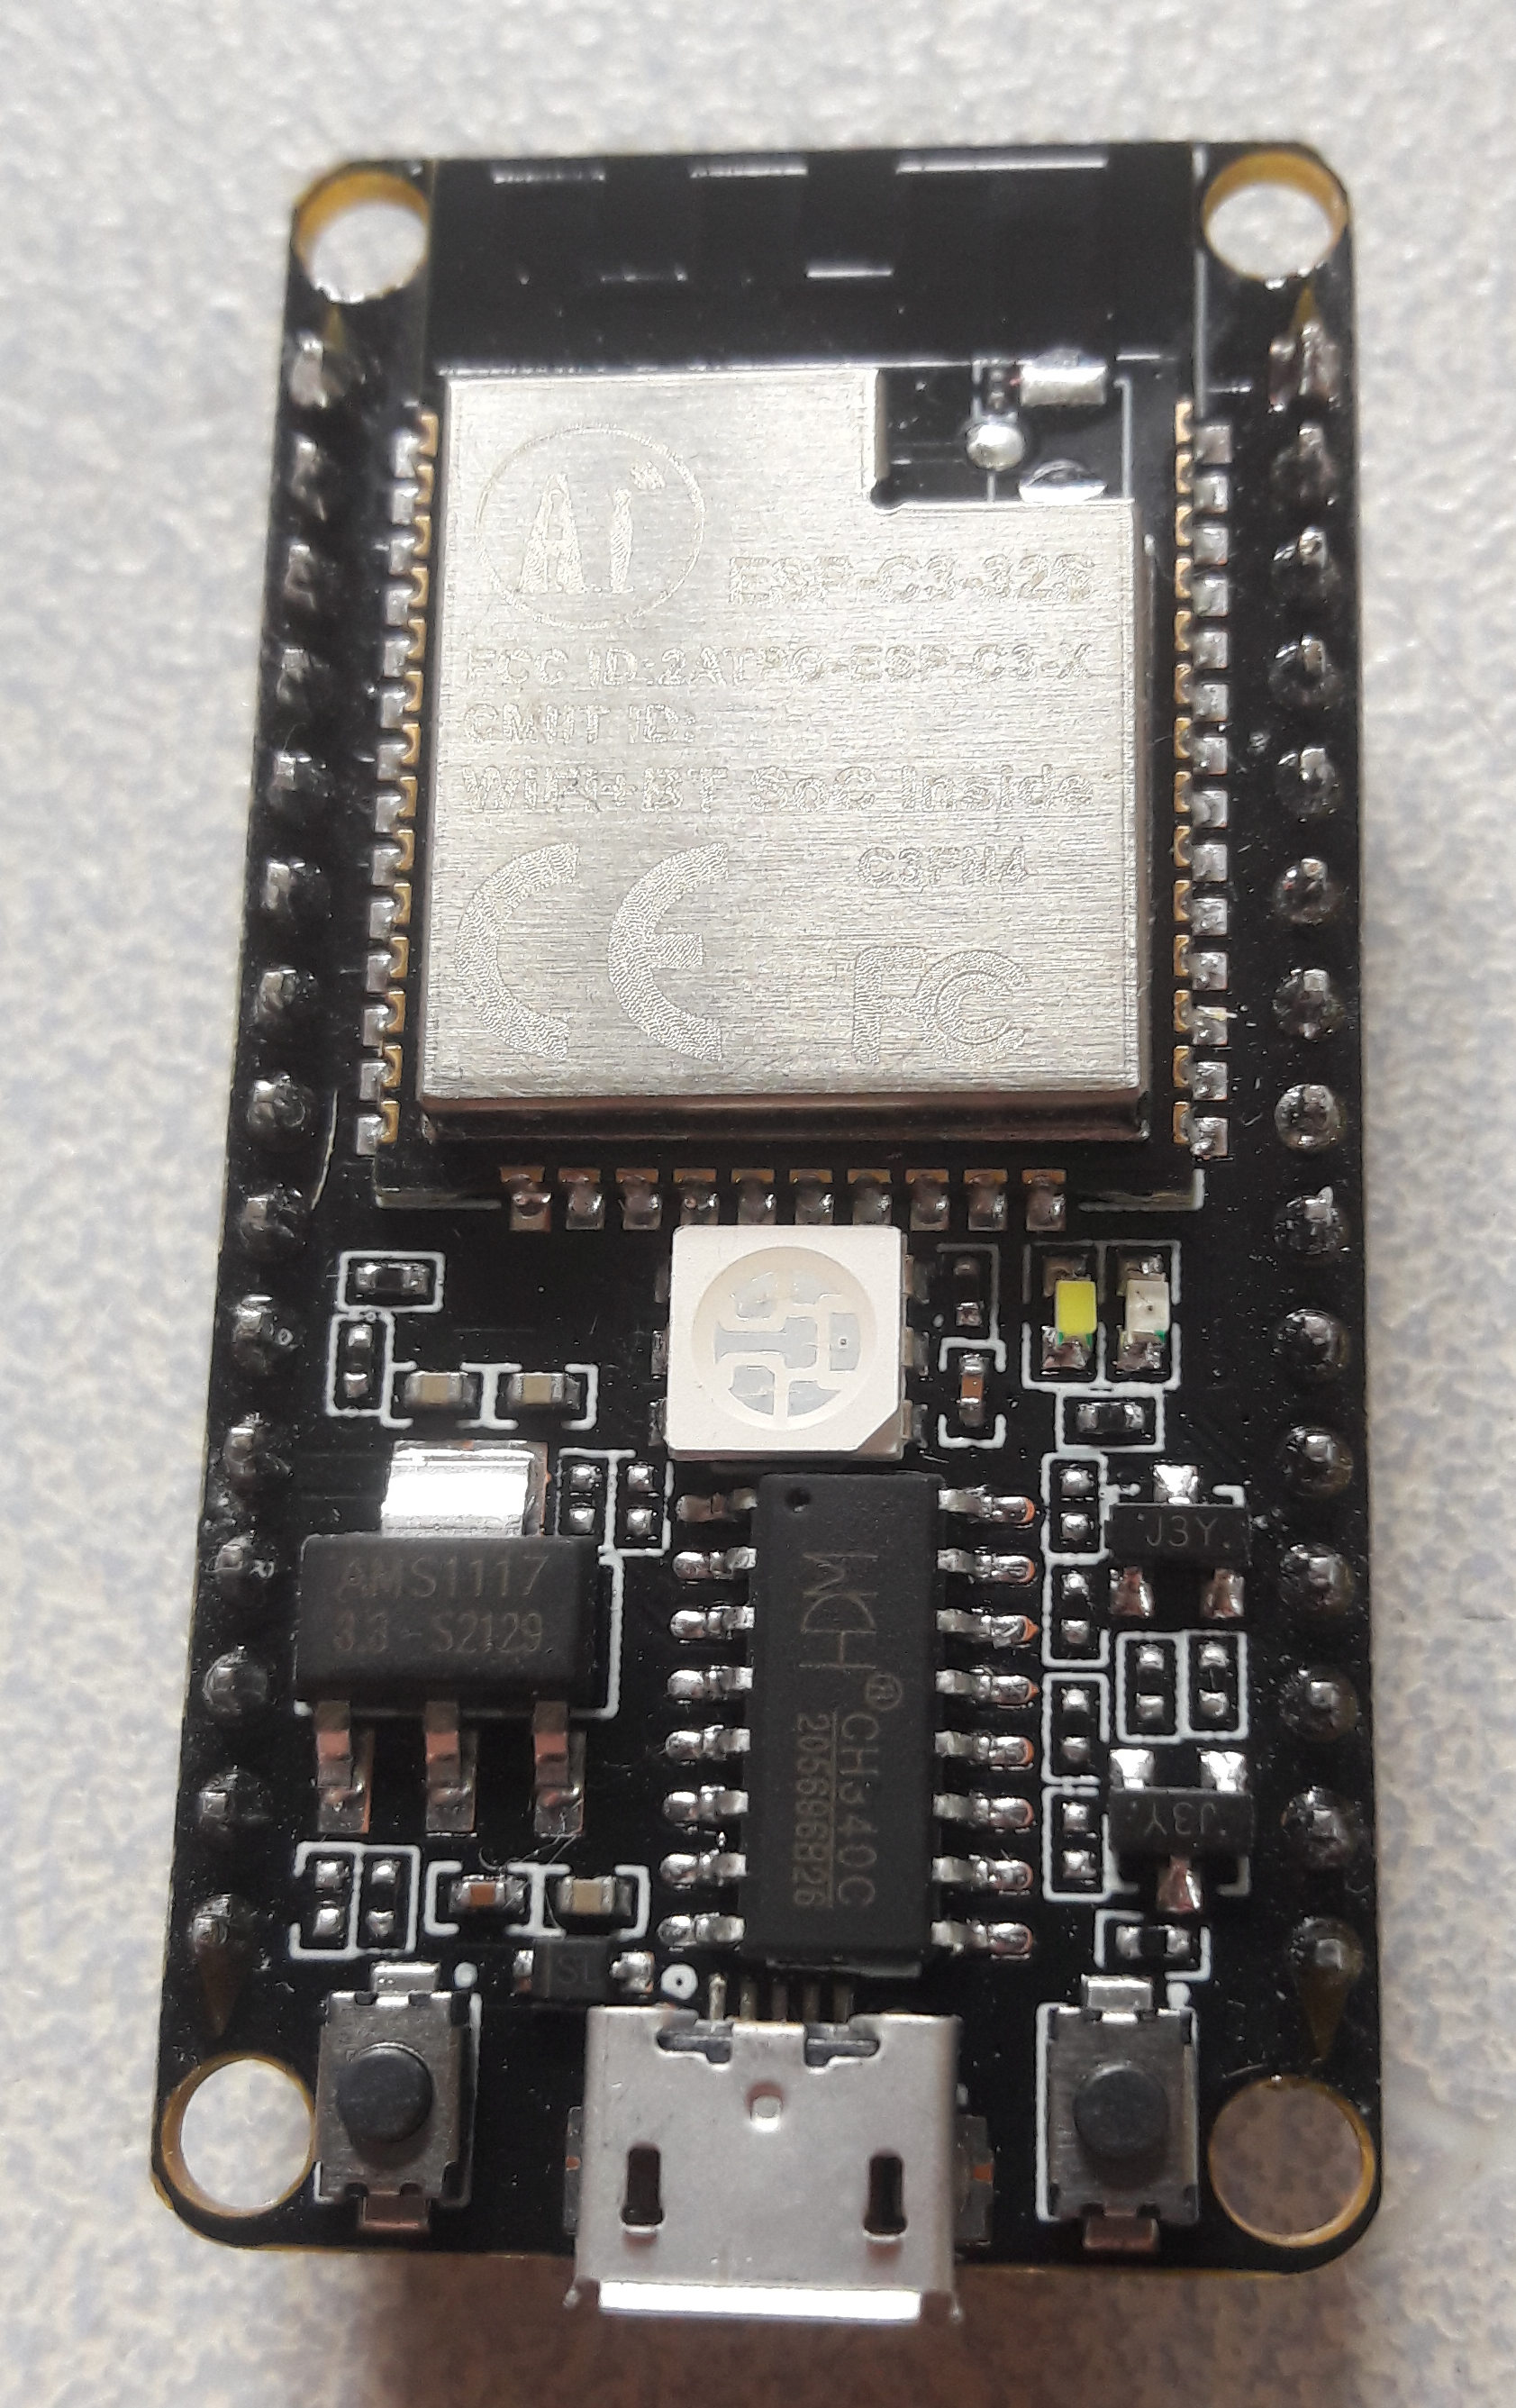
\includegraphics[width=0.3\paperwidth]{images/esp32-board}
        \caption{ESP32 en una tarjeta NodeMCU} \footnotesize
        Fuente: \textit{Wikipedia} $\mid$ ESP32. By Popolon - Own work, CC BY-SA 4.0, https://commons.wikimedia.org/w/index.php?curid=112634884.
    \end{figure}

    \subsection{Características}

    Las especificaciones completas de la tarjeta ESP32 se encuentran el la \href{https://www.espressif.com/sites/default/files/documentation/esp32_datasheet_en.pdf}{hoja de especificaciones} oficial, por lo que se enunciarán las características más destacables del producto a continuación \cite{espressif-systems-shanghai-co-ltd-2022B}:

    \begin{itemize}
        \item Wi-Fi 802.11 b/g/n, 802.11 n ($2.4GHz)$ hasta $150Mbps$, diversidad de antena, etc.

        \item Bluetooth v4.2 BR/EDR y LE, transmisor clase-1, clase-2, clase-3 sin amplificador de potencia externo, control de potencia, +9 dBm de transmisión, etc.

        \item CPU Xtensa single-/dual-core $32 bit$ LX6.

        \item $448 KB$ de ROM.

        \item $520 KB$ de SRAM.

        \item $16 KB$ de SRAM en RTC.

        \item Oscilador inteno de $8 MHz$ con calibración.

        \item Oscilador RC interno con calibración.

        \item Un timer RTC, etc.

        \item $34$ GPIO programables.

        \item Boot seguro, encriptación mediante flash, algoritmos AES, SHA-2, RSA, ECC, RNG.

        \item Gran cantidad de aplicaciones como cámaras para streaming de video, robots para agricultura, reconocimiento de imágen, etc.
    \end{itemize}

    Las características son sin lugar a duda muy interesantes y completas. En tanto a las aplicaciones que se le pueden dar a este microcontrolador, son muchísimas.

    \bigbreak

    En el siguiente diagrama de bloques, se puede visualizar la arquitectura de esta tarjeta donde se destacan las características principales:

    \begin{figure}[H]
        \centering
        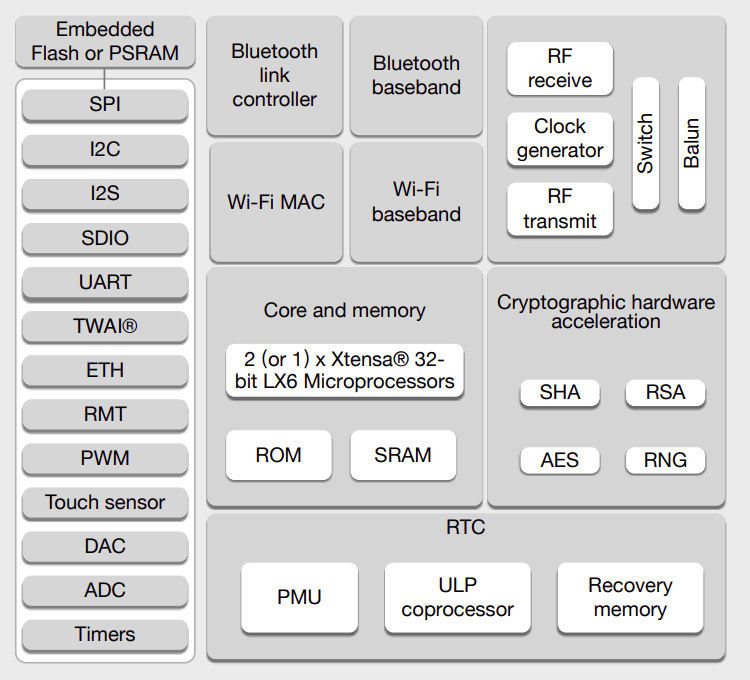
\includegraphics[width=0.3\paperwidth]{images/esp32-functional-block-diagram}
        \caption{ESP32 diagrama de bloque funcional} \footnotesize
        Fuente: \textit{ESPRESSIF} $\mid$ ESP32 Datasheet \cite{espressif-systems-shanghai-co-ltd-2022B} (bajo uso justo)
    \end{figure}

    O también, en esta otra la cual comparte mucha similitud:

    \begin{figure}[H]
        \centering
        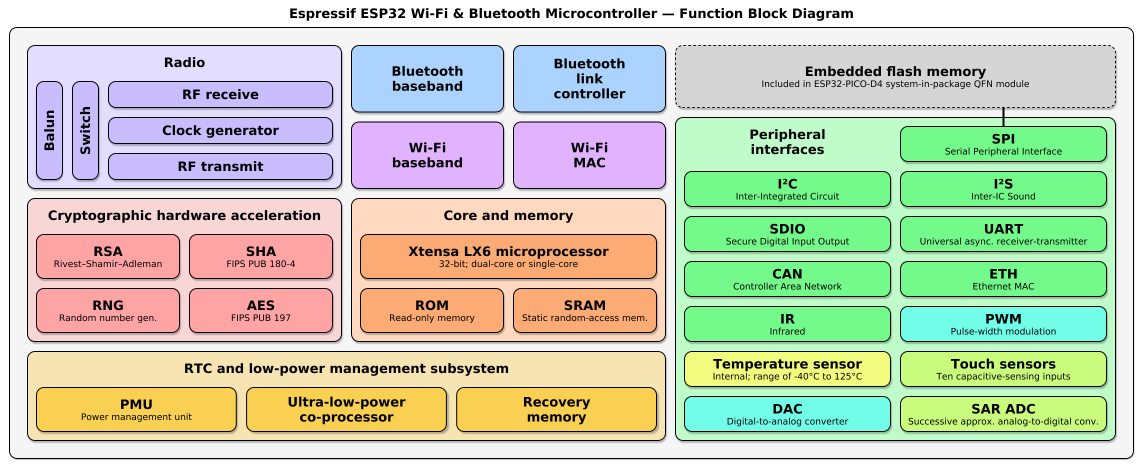
\includegraphics[width=0.3\paperwidth]{images/espressif-esp32-chip-function-block-diagram}
        \caption{ESP32 diagrama de bloque funcional (figura opcional)} \footnotesize
        Fuente: \textit{Wikipedia} $\mid$ ESP32. By Brian Krent (talk · contribs) - Own work, CC0, https://commons.wikimedia.org/w/index.php?curid=72304119.
\end{figure}

Para poder hacer uso del dispositivo, es importante saber su disposición de pines, esto se obtiene de la siguiente documentación oficial:

\begin{figure}[H]
\centering
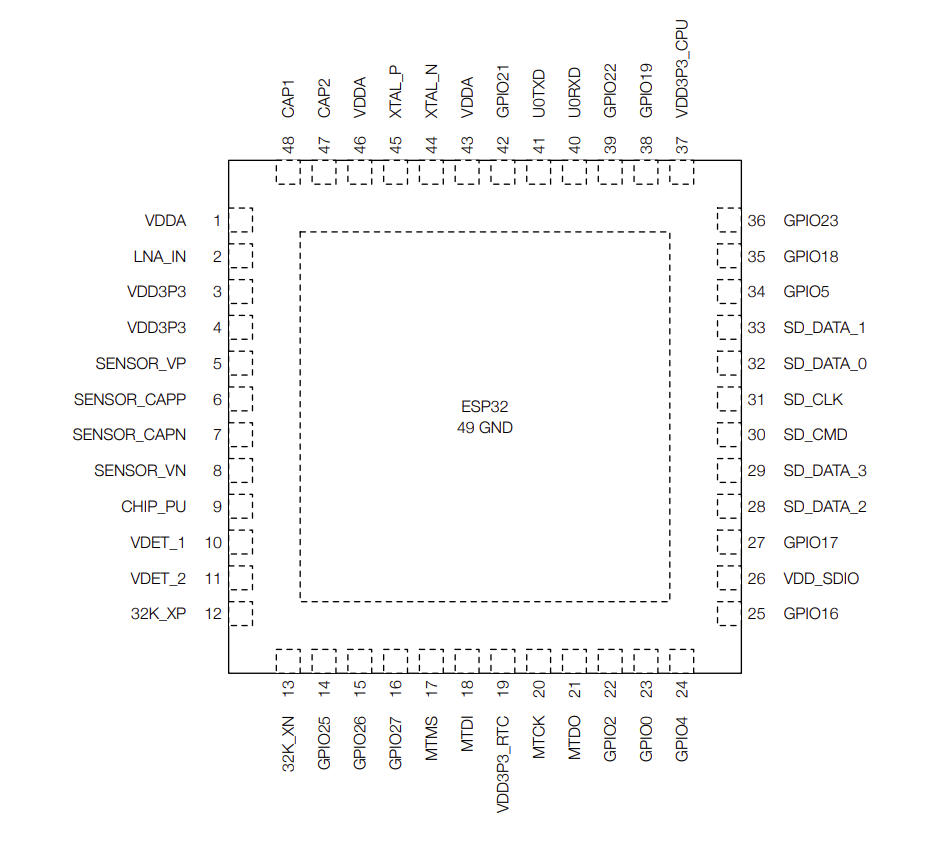
\includegraphics[width=0.3\paperwidth]{images/esp32-pin-layout.png}
\caption{ESP32 layout de pines (QFN 6*6, Vista desde arriba)} \footnotesize
Fuente: \textit{ESPRESSIF} $\mid$ ESP32 Datasheet \cite{espressif-systems-shanghai-co-ltd-2022B} (bajo uso justo)
\end{figure}

Por último, en \href{http://esp32.net}{http://esp32.net} se encuentran también características y especificaciones, recursos de desarrollo para muchos lenguajes de programación y plataformas, comunidades en línea sobre este dispositivo en específico, lecturas y videos, plataformas de hardware, información sobre proveedores que venden este dispositivo y otros accesorios \cite{esp32net-esp32net-iot}.

\section{}




\section{Conclusión}\label{sec:conclusion}




\printbibliography

\end{document}
